\selectlanguage{spanish}
\let\textcircled=\pgftextcircled
\chapter {Resultados}
\label{chap:resultados}

\initial{L}os métodos propuestos para la estimación de tiempo de viaje, aplicados a observaciones GPS y Bluetooth, fueron evaluados a través de diferentes enfoques, incluyendo un análisis cuantitativo y una discusión general de la calidad de los métodos presentados, considerando además, la caracterización de la señal Bluetooth.

El objetivo de utilizar estos métodos es medir el tiempo de viaje y compararlo con el tiempo real de la simulación. Las evaluaciones se realizan sobre la red de ejemplo \(\mathcal{G}\), representada por la figura \ref{fig:result-network}. La red cuenta con junciones internas que separan la calle en tramos (o cuadras) de aproximadamente 200 metros cada uno y, en los extremos de la red, se encuentran los distritos que se utilizan para modelar la demanda. Por otro lado, los identificadores corresponden a la nomenclatura que llevan los arcos originales de la red en el simulador \textit{SUMO}. En la red se despliegan Monitores Bluetooth de igual modo a como fueron utilizados para la simulación de detecciones. En la simulación, todos los monitores fueron configurados para  realizar detecciones hasta 100 metros de distancia entre un vehículo y el detector.

\begin{figure}[!htp]
\begin{minipage}{.49\textwidth}
	\centering
	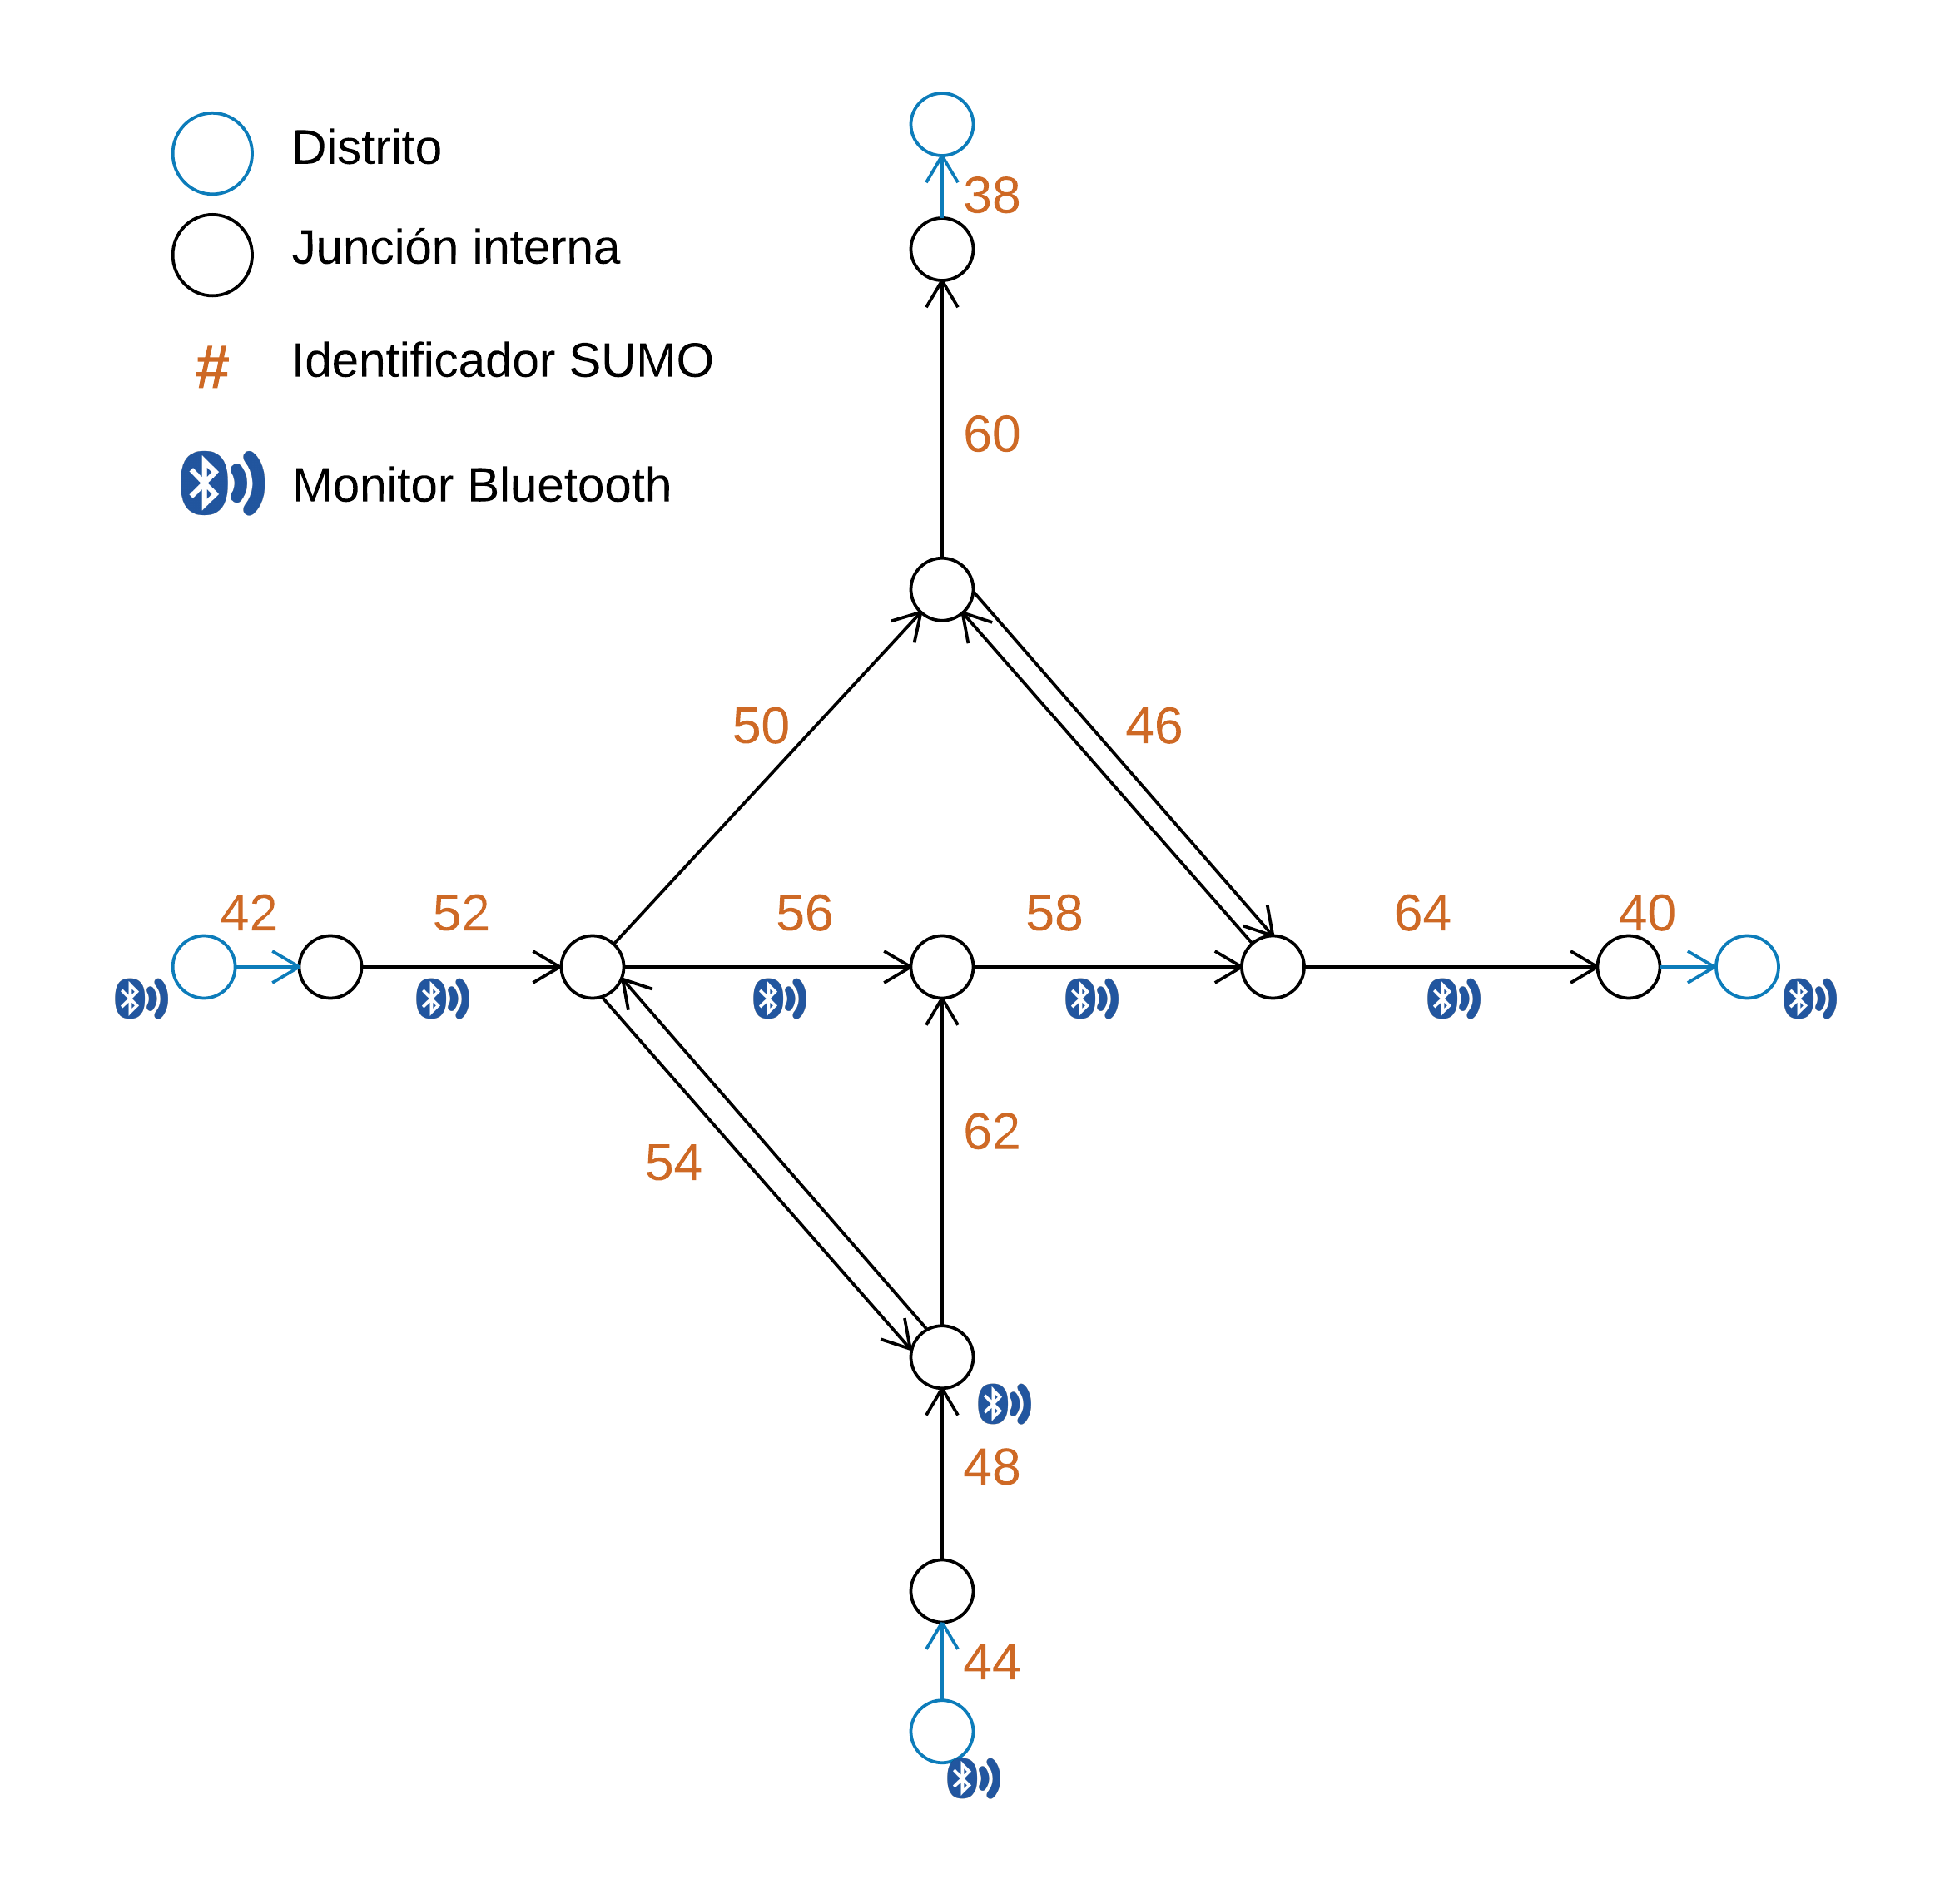
\includegraphics[width=0.9\linewidth]{images/result-network.png}
	\captionsetup{width=0.8\linewidth}
	\caption{Red de calles para las pruebas de la plataforma.}
    \label{fig:result-network}
\end{minipage}
\begin{minipage}{.49\textwidth}
	\centering
	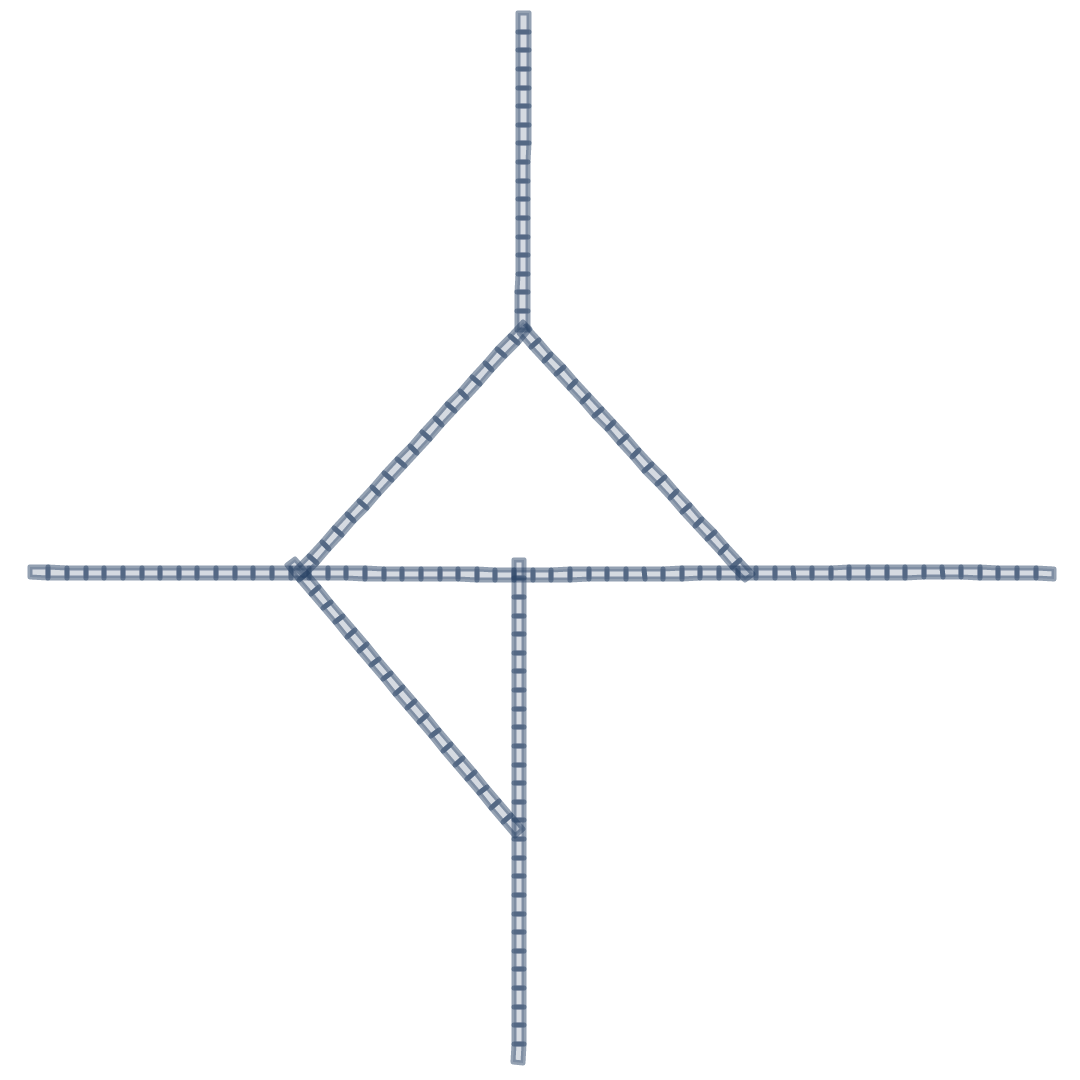
\includegraphics[width=0.9\linewidth]{images/result-segmentos.png}
	\captionsetup{width=0.8\linewidth}
	\caption{División de la red en segmentos (\textit{SegmentoViterbi}).}
    \label{fig:result-segments}
\end{minipage}
\end{figure}

Para la ejecución del algoritmo de estimación, los segmentos son divididos aplicando la metodología propuesta en el apartado \ref{ssec:hmm-shortsegments}, formando \(\mathcal{G'}=<\mathcal{V'},\mathcal{E'} >\), con un total de 154 estados $\mathcal{V'}$ (Figura \ref{fig:result-segments}).

Se establecen dos recorridos $R1$ y $R2$ de longitud $l=1.22$ km. Se realizan simulaciones para ambos recorridos, variando los parámetros índice de penetración y probabilidad de observación. Finalmente se realizan pruebas sobre los recorridos $R1$ y $R2$ conjuntamente.

\begin{figure}[!htp]
	\centering
	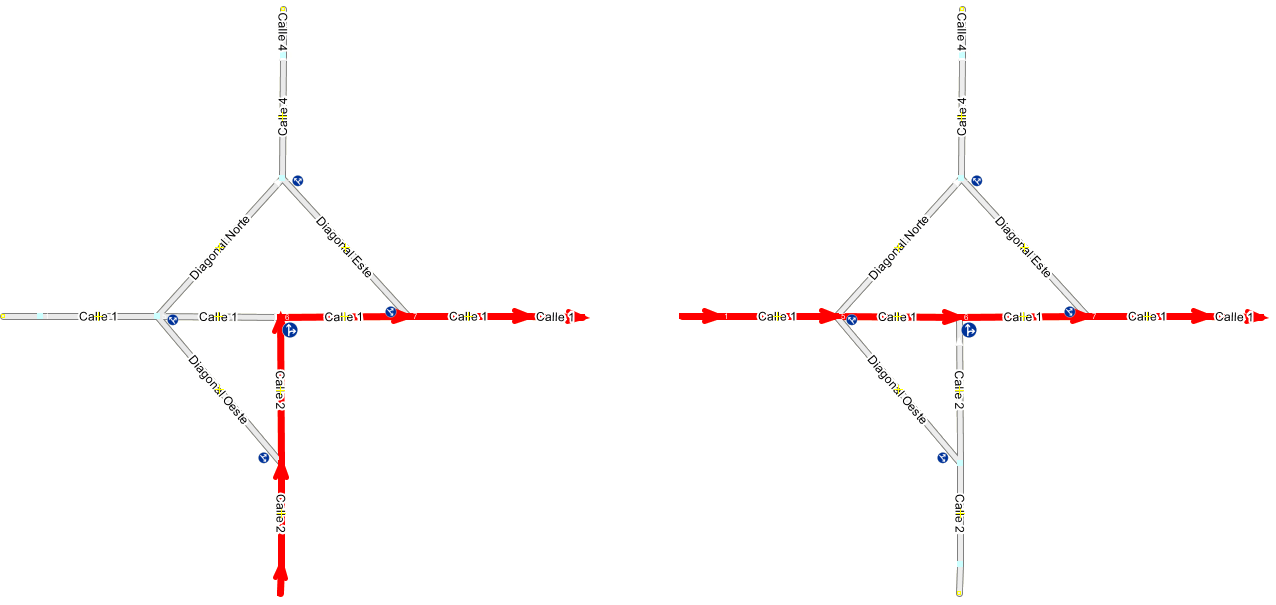
\includegraphics[width=0.9\linewidth]{images/result-r1r2.png}
	\captionsetup{width=0.8\linewidth}
	\caption{Recorridos definidos R1 y R2, respectivamente..}
    \label{fig:result-r1r2}
\end{figure}

\section{Estimación GPS}

En el caso de observaciones GPS, \textit{SUMO} arroja posiciones en cada ciclo de simulación (Figura \ref{fig:result-pobs-pf} - A) y sobre estas se aplican dos procesos. En primer lugar, se descartan observaciones con cierta probabilidad $p_{obs}$ (B)y, en segundo lugar, se modela el error de una observación como una variable aleatoria $X$ distribuida normalmente con media cero y desvío dado (C, D y E).

\begin{figure}[!htp]
	\centering
	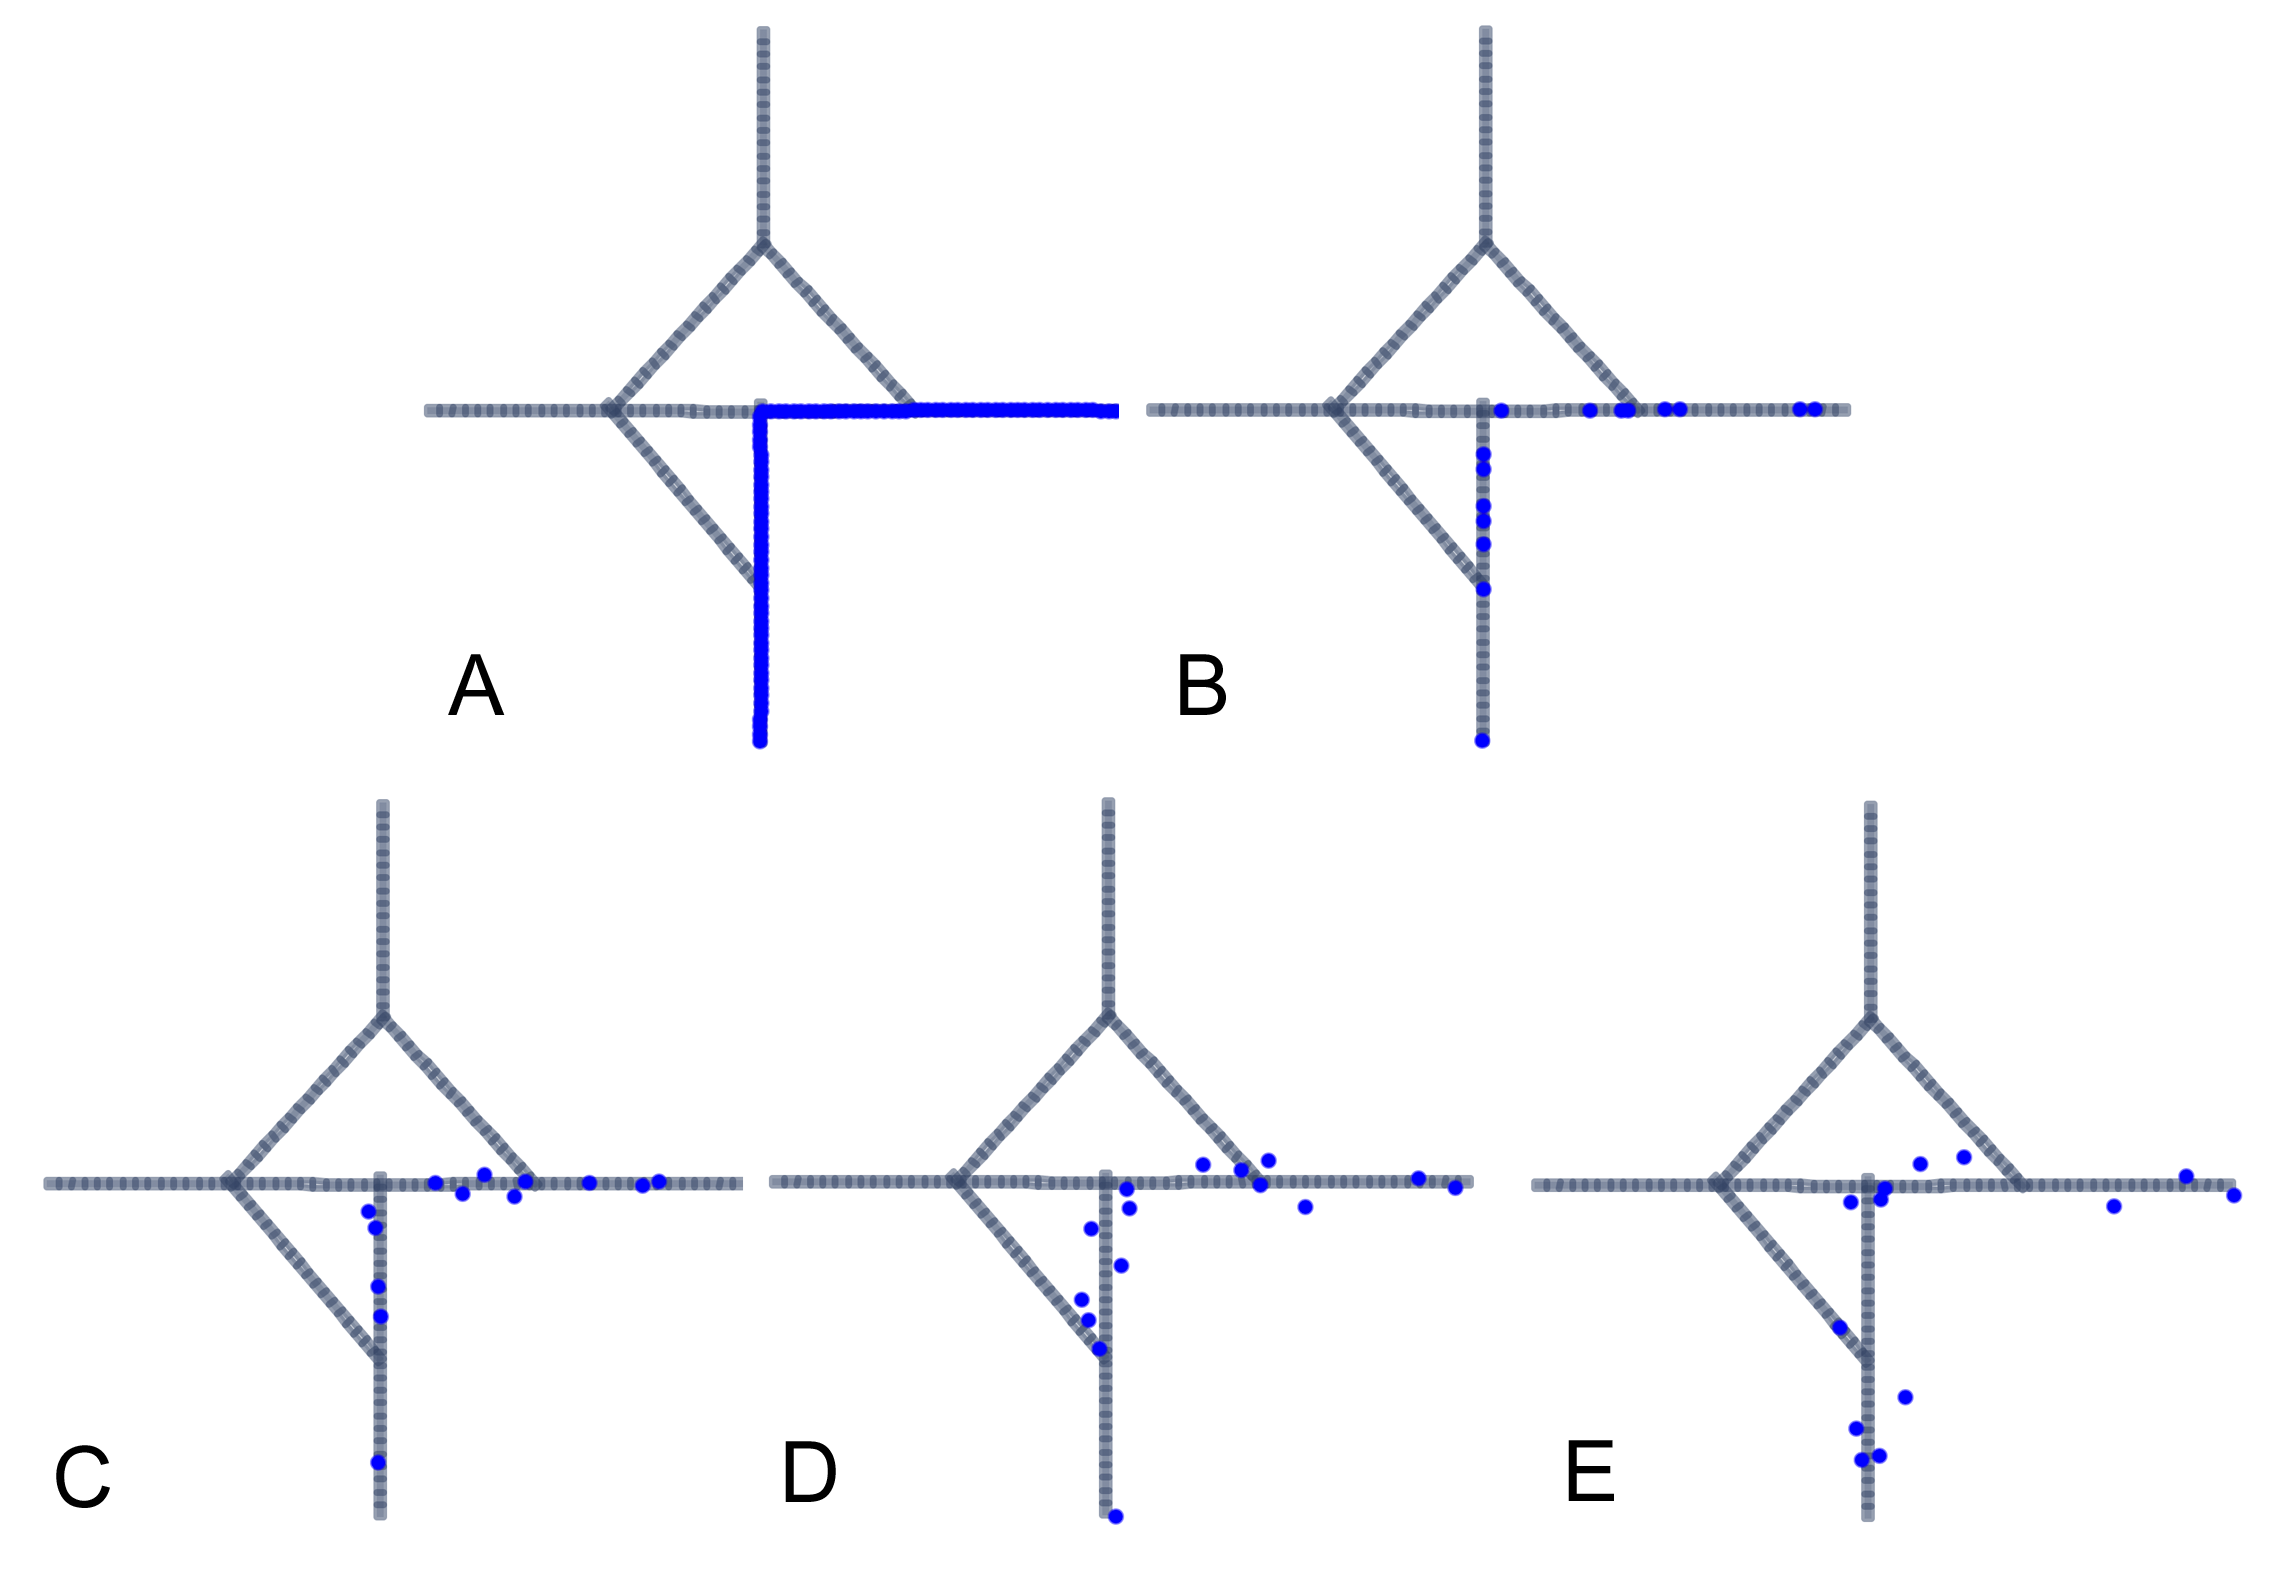
\includegraphics[width=0.9\linewidth]{images/result-pobspf.png}
	\captionsetup{width=0.8\linewidth}
	\caption{Recorrido simulado para 1 vehículo en el recorrido R1, con probabilidades de obsevación: $p_{obs}=1$ (A) y $p_{obs}=0.125$ (B); a partir de simulaciones con $p_{obs}=0.125$ se visualizan perturbaciones de: $PF=\{1, 5, 10\}$ (C, D y E, respectivamente) }
    \label{fig:result-pobs-pf}
\end{figure}

Luego, el algoritmo estima una secuencia de estados que describe la trayectoria más probable $\tau_{opt}$ dada la secuencia de observaciones \(\mathcal{P}\). Se considera como ground truth a todos los segmentos recorridos por la secuencia original \(\mathcal{T}\).

Para las comparaciones se tendrán en cuenta los siguientes aspectos:

\begin{itemize}
    \item Tiempo de viaje medio por tramo.
    \item Relación tiempo - segmento.
\end{itemize}

A partir de la secuencia de estados $\tau_{opt}$, se determina el tiempo de viaje medio por segmento. Esto es, por ejemplo, si un vehículo se traslada por los segmentos 1, 2 y 3 con la frecuencia:
\begin{align*}
\tau_{opt} = \{1, 1, 2, 3, 3\},
\end{align*}
como resultado se tiene que el vehículo demoró dos segundos en el segmento 1, un segundo en el segmento 2 y dos segundos en el segmento 3. Éste cálculo se corresponde con la frecuencia absoluta de las detecciones en cada segmento $F_i$. Se realiza para todos los vehículos, tomando el valor medio de cada segmento. Luego, se agrupan las demoras obtenidas según el tramo al que pertenece cada segmento. El tiempo de viaje estimado en cada tramo $e$ ($TTEst_e$, por sus siglas en inglés: Estimated Travel Time) se calcula a partir de la suma de las demoras de cada segmento $s \in S$ tal que $s$ surge de la división del tramo $e$.
\begin{align}
TTEst_e = \sum_{i=1}^S SegmentTT_i
\end{align}

El tiempo de viaje en cada segmento es, entonces, la relación entre la suma de la frecuencia absoluta de cada estado $F_i$ y el total de vehículos $V$, o bien:
\begin{align}
SegmentTT_i = \frac{\sum F_i}{V}
\end{align}

A continuación se detallan las series de simulación para los recorridos $R1$ y $R2$. En primera instancia se muestran las distancias y tiempos totales para cada recorrido y, luego, se analizan los resultados desde otra perspectiva, analizando los tiempos por cada tramo.

\begin{itemize}
\item $P_{obs}$: Probabilidad de observación (o probabilidad de lectura), es la probabilidad de que un vehículo realice una transmisión dada su ubicación.
\item PR: Índice de penetración, se corresponde con el porcentaje de vehículos que portan un dispositivo de posicionamiento.
\item DistSim: Distancia recorrida por simulación (m).
\item DistEst: Distancia Estimada (m).
\item TTEst: Tiempo de viaje total estimado por edge (s).
\item TTSim: Tiempo de viaje total Simulado (s)
\item VelSim: Velocidad media Simulado (m/s)
\item VelEst: Velocidad media Estimada (m/s)
\item PF: Factor de perturbación.
\item Veh: Cantidad de vehículos observados.
\end{itemize}

\begin{table}
\centering
\begingroup\catcode`"=9
\csvreader[
tabular=>{\itshape}llllllll>{\ttfamily}l,
table head=\toprule\Header{Recorrido} & \Header{Pobs} & \Header{PF}  & \Header{TTSim} & \Header{TTEst}  & \Header{DistSim} & \Header{DistEst} & \Header{VelSim} & \Header{VelEst} \\\midrule,
table foot=\bottomrule]
{reports/r1-1v.csv}{}{\csvlinetotablerow}
 \captionsetup{width=0.8\textwidth}
    \caption{Resultados de tiempos y distancias en la simulación de un vehículo, sobre el recorrido R1, aplicando el Método 1}
    \label{tbl:r1-1v}
\endgroup
\end{table}

En la tabla \ref{tbl:r1-1v} se detallan los resultados de la aplicación del método 1 sobre la simulación de un vehículo en el recorrido R1, variando los parámetros $p_{obs}$ y el factor de perturbación $PF$. Aquí, los tiempos coinciden entre los casos simulados y estimados porque se obtienen a partir de la diferencia entre las marcas de tiempo de la primera y última observación. Las distancias \textbf{estimadas} se corresponden con la distancia que abarcan los estados (segmentos) resultantes; en otras palabras, los valores de distancia serán múltiplos de la longitud del segmento $l = 22.22$ m. Finalmente, podemos observar una comparación de las velocidades medias obtenidas en la Figura \ref{fig:speed-r1-1v}. La diferencia máxima registrada es de 0.16 m/s.

\begin{figure}[!htp]
	\centering
	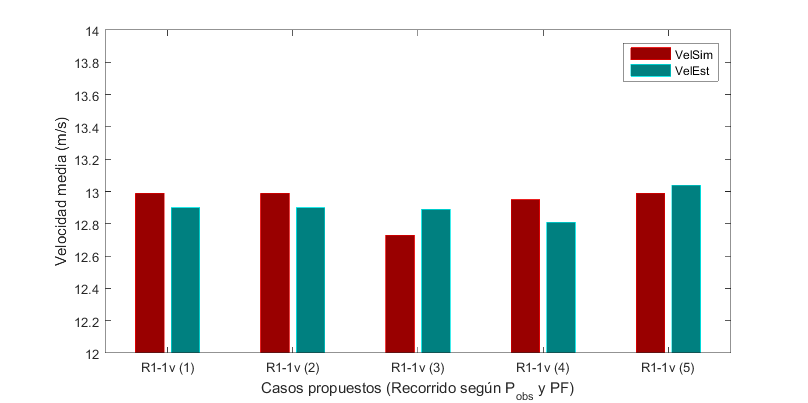
\includegraphics[width=0.7\linewidth]{images/speed-r1-1v.png}
	\captionsetup{width=0.7\linewidth}
	\caption{Estimación de la velocidad media general para las variaciones de parámetros $p_{obs}$ y $PF$ sobre el recorrido R1}
    \label{fig:speed-r1-1v}
\end{figure}

Es importante considerar otros aspectos en el análisis de las estimaciones. Para el estudio de los tiempos de viaje sobre los tramos (cuadras) de la red original, se utilizan valores agregados (promedios) de las demoras estimadas. En la Figura \ref{fig:edge-tt-r2} se muestran los resultados para el tiempo de viaje estimado por tramos (cuadras o \textit{edges}) para 10, 100 y 200 vehículos, respectivamente. 

\begin{figure}[!htp]
	\centering
	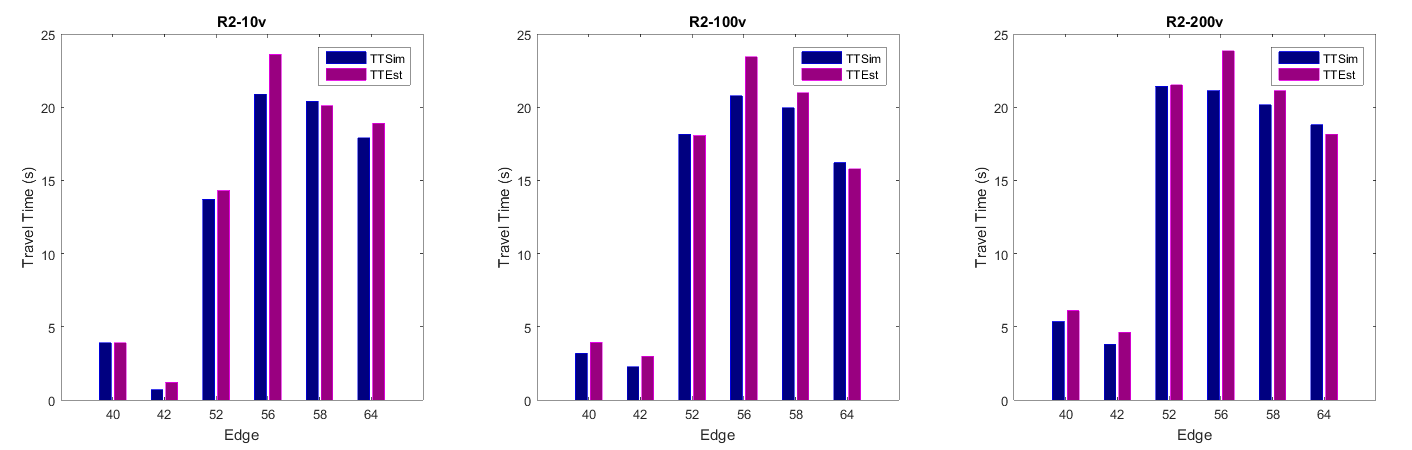
\includegraphics[width=\linewidth]{images/edge-tt-r2.png}
	\captionsetup{width=0.8\linewidth}
	\caption{Estimación del Tiempo de Viaje para 10, 100 y 200 vehículos en el recorrido R2, con $p_{obs}=0.125$ y $PF=10$}
    \label{fig:edge-tt-r2}
\end{figure}

Recordando la estructura original de la red $\mathcal{G}$, puede observarse que los arcos que presentan mayor error (Edge 40 y Edge 44) son los que corresponden a los distritos para modelar la demanda. En estas zonas de pequeña longitud es donde comienzan a ingresar y retirarse los vehículos simulados. Por lo mencionado anteriormente, el tiempo de viaje asignado a estos tramos es más corto respecto a los demás. En términos generales, se obtuvo un error máximo de 2.72 segundos en el Edge número 56 en la simulación de 200 vehículos.

Finalmente, se incluye un cuadro comparativo entre los métodos propuestos.

\begin{table}[!htp]
\centering
\begingroup\catcode`"=9
\csvreader[
tabular=>{\itshape}llll>{\ttfamily}l,
table head=\toprule\Header{Método} & \Header{Recorrido} & \Header{$P_{obs}$}  & \Header{PF} & \Header{Error Medio (seg)}  \\\midrule,
table foot=\bottomrule]
{reports/method-compare.csv}{}{\csvlinetotablerow}
 \captionsetup{width=0.8\textwidth}
    \caption{Cuadro comparativo del error medio en la estimación del Tiempo de Viaje (TT) obtenido en simulaciones para 10 vehículos, en los recorridos 1 y 2, estimadas a partir de los métodos 1 y 2.}
    \label{tbl:method-compare}
\endgroup
\end{table}


\section{Estimación Bluetooth}

En el caso de las estimaciones Bluetooth, se valida el funcionamiento del modelo planteado y se compara con la estimación obtenida a partir de la caracterización de la señal BT.

Como se mencionó en la introducción del trabajo, en un caso ideal, la potencia de señal recibida en función de la distancia puede modelarse a través de la ecuación de transmisión de Friis. Aquí, se aplica la misma metodología desarrollada para la estimación de las funciones de densidad $opdf$, pero, en lugar de utilizar las muestras experimentales, se evalúa una función $P_r(d) = friis(d)$ en el intervalo $(0 100]$ y se clasifica cada valor $P_r$ según la distancia en grupo de a 5 metros. Por ejemplo, se clasificarán las señales \{friis(1), friis(2),..., friis(5)\} como distancia 5, el siguiente grupo será de distancia 10, y así sucesivamente.

En la Figura \ref{fig:edge-tt-bt} se muestran tiempos de viaje obtenidos por estimación basada en la ecuación de transmisión de Friis. De modo similar se obtuvo la simulación de la intensidad de señal recibida: evaluando  la ecuación con las distancias entre el vehículo simulado y cada monitor.

\begin{figure}[!htp]
	\centering
	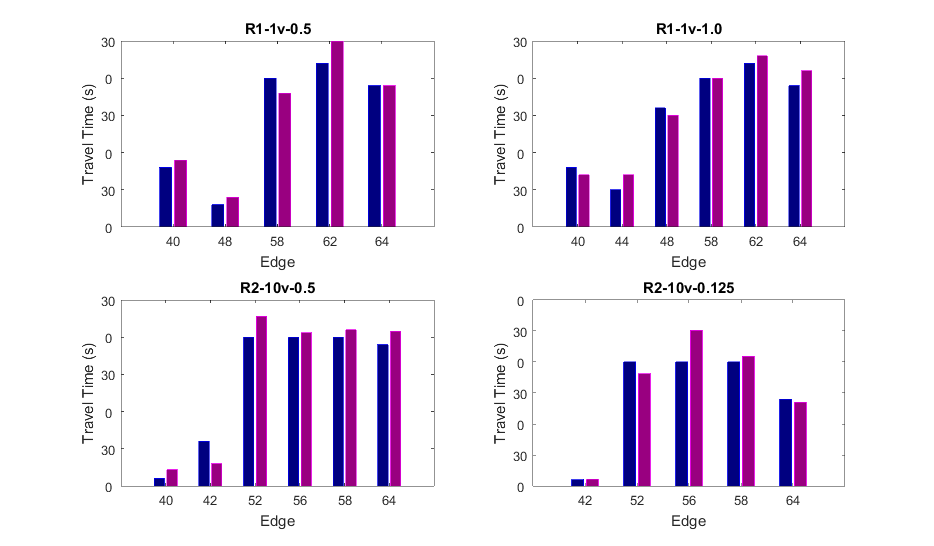
\includegraphics[width=0.9\linewidth]{images/edge-tt-bt.png}
	\captionsetup{width=0.8\linewidth}
	\caption{Estimación del Tiempo de Viaje vía detección Bluetooth para 10 vehículos en el recorrido R1 y R2, con diferentes combinaciones de $p_{obs}$}
    \label{fig:edge-tt-bt}
\end{figure}


La Figura \ref{fig:time-segment} representa el avance de un vehículo sobre los segmentos (eje vertical) a lo largo del tiempo (eje horizontal). En este caso, se trata de un único vehículo en el recorrido 1, y la diferencia media entre tiempo simulado y tiempo estimado entre segmentos es de apenas 1 segundo, validando de esta forma la metodología utilizada.

\begin{figure}[!htp]
	\centering
	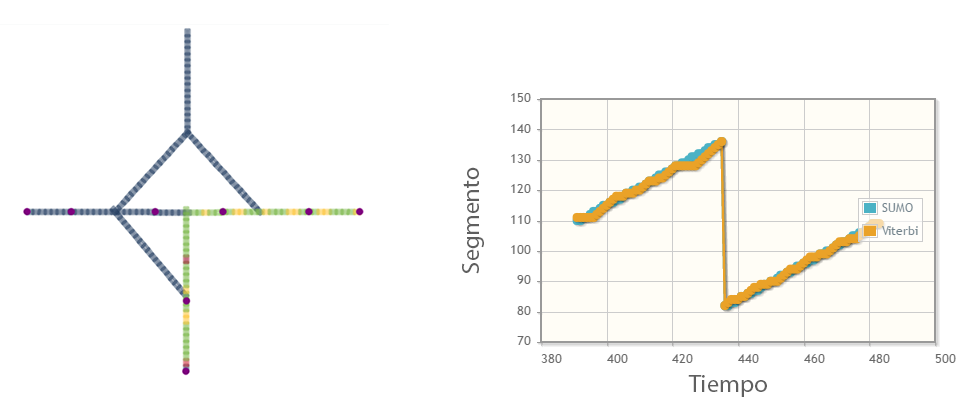
\includegraphics[width=0.7\linewidth]{images/time-segment.png}
	\captionsetup{width=0.8\linewidth}
	\caption{Estimación del Tiempo de Viaje vía detección Bluetooth para 1 y 10 vehículos en el recorrido R1 y R2, con diferentes combinaciones de $p_{obs}$}
    \label{fig:time-segment}
\end{figure}

Finalmente, se realiza una comparación del tiempo de viaje estimado a partir la caracterización experimental de la señal de Bluetooth. Se observan valores para distintas probabilidades de lectura $p_{obs}$, sobre el trayecto de un vehículo en el recorrido 2, utilizando el método de simulación Bluetooth por perturbación (segundo método de simulación). Aquí se utilizan las medidas experimentales para generar observaciones aleatorias con el error medio observado en el estudio realizado.

\begin{table}
\centering
\begingroup\catcode`"=9
\csvreader[
tabular=>{\itshape}llll>{\ttfamily}l,
table head=\toprule\Header{Edge} & \Header{TTSim} & \Header{TTEst-1} & \Header{TTEst-0.8}  & \Header{TTEst-0.5}  \\\midrule,
table foot=\bottomrule]
{reports/TTEst-bt-perturbacion.csv}{}{\csvlinetotablerow}
 \captionsetup{width=0.8\textwidth}
    \caption{Tiempos de viaje estimados para 1 vehículo en el Recorrido 2, a distintos valores de $p_{obs}$.}
    \label{tbl:tte-btperturbacion}
\endgroup
\end{table}

Analizando el cuadro \ref{tbl:tte-btperturbacion}, se percibe un error máximo de 5 segundos y un error medio máximo de 1.75 segundos. Lo cual es relativamente bajo respecto al tiempo de viaje real de cada tramo en el recorrido (menor al 8\%). Cabe destacar que el filtro $p_{obs}=0.5$ arroja alrededor de 30 detecciones entre los 6 monitores de la red y, en las pruebas de velocidad, se observaron como mínimo 5 detecciones por monitor (a 80 Km/h), por lo cual, la probabilidad de lectura indicada permite tener un tamaño de muestra comparable a la realidad.
\par 

%\begin{tabular}{*5l}    \toprule
%\emph{Error medio} & \emph{foo} &&&  \\\midrule
%1.75 s    & A  & B  & C  & D  \\ 
%Model $X$ & X1 & X2 & X3 & X4\\\bottomrule
% \hline
%\end{tabular}